\documentclass[preview]{standalone}

\usepackage{amsmath}
\usepackage{amssymb}
\usepackage{stellar}
\usepackage{bettelini}

\hypersetup{
    colorlinks=true,
    linkcolor=black,
    urlcolor=blue,
    pdftitle={Biologia},
    pdfpagemode=FullScreen,
}

\begin{document}

\title{Biologia}
\id{biologia-ciclo-carbonio}
\genpage

\begin{snippetdefinition}{serbatoio-abiotico-definition}{Serbatoio abiotico}
    Il \textit{serbatoio abiotico} 
    è il posto dove si trova la maggior parte dell'elemento in forma abiotica,
    quindi in forma inorganica.
\end{snippetdefinition}

\plain{Il carbonio si trova principalmente nelle roccie e negli oceani.}

\begin{snippet}{ciclo-biogeochimico-illustration}
    \begin{center}
    \begin{figure}[th]
        \centering
        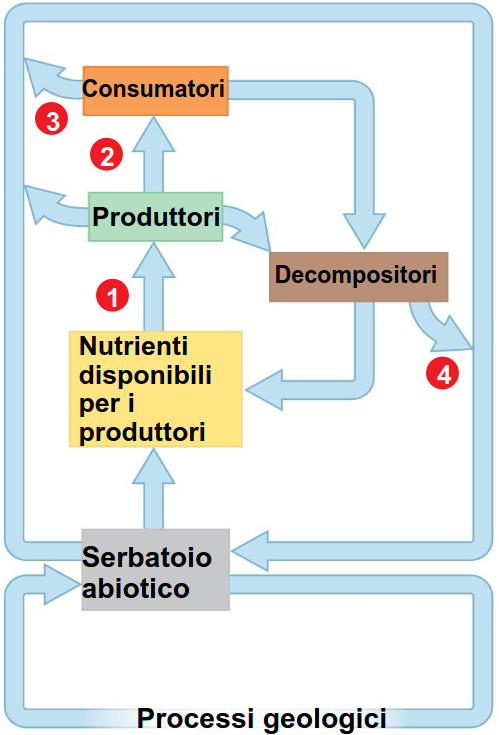
\includegraphics[width=0.6\textwidth]{./resources/ciclo_biogeochimico.png}
    \end{figure}
    \end{center}
\end{snippet}

\begin{snippet}{4f77f367-52aa-4c81-a90f-2d6388479017}
    \begin{enumerate}
        \item Assimilazione dei nutrienti da parte dei produttori, come ad esempio la fotosintesi nel ciclo del carbonio. 
        \item Catena alimentare, passa da un livello trofico all'altro. 
        \item Scarti prodotti dagli organismi della rete alimentare; a sinistra dalla respirazione cellulare (CO2), mentre la freccia destra da scarti organici (feci e urine) oppure gli organismi stessi, che ad esempio muoiono.
        \item può essere direttamente convertita in CO2, quindi sono gli scarti dei decompositori
    \end{enumerate}
    
    Il carbonio può essere trasformato dalla fotosintesi, successivamente 
    respirazione cellulare, fermentazione, decomposizione, combustione e sedimentazione (senza O2).
\end{snippet}

\end{document}